113. \begin{figure}[ht!]
\center{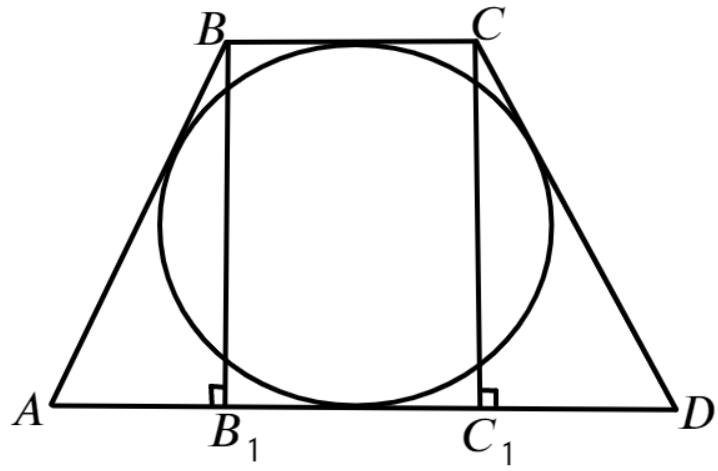
\includegraphics[scale=0.35]{g9-113.png}}
\end{figure}\\
Если трапеция описанная, суммы её противоположных сторон равны, поэтому $AB=CD=\cfrac{4+9}{2}=\cfrac{13}{2}.$ Опустим высоты $BB_1$ и $CC_1,$ тогда $AB_1=C_1D=\cfrac{9-4}{2}=\cfrac{5}{2}$ и $BB_1=\sqrt{\cfrac{169}{4}-\cfrac{25}{4}}=6.$ Радиус вписанной окружности равен половине высоты, поэтому $R=6:2=3.$\newpage\noindent
